\documentclass[12pt]{article}

\usepackage{amsmath,amsthm,amssymb,xcolor,graphicx,tikz,listings}
\usepackage{comment}
\usepackage{cite}
\usepackage[T1]{fontenc}
\usepackage[utf8x]{inputenc}
\usepackage[pdftex]{hyperref}
\usetikzlibrary{positioning}

\begin{document}

% Macros
%------------------------------------------------------------
\def\Any {{\mathcal U}}
\def\Prop{{\mathcal P}}
\def\Indsort{{\Any_\mathcal I}}
\def\Fixsort{{\Any_\mathcal F}}
\def\Uni {{\mathcal L}}
\def\Univ {{\mathcal L}}
\def\Top {{\Any_\infty}}

\def\Nat{{\mathbb N}}

\def\case{{\text{\it case}}}
\def\ctree{{\text{\it tree}}}
\def\ct#1{{\mathcal #1}}
\def\cta {{\text{cta}}}
\def\fix {{\text{\it fix}}}
\def\fspinetree{{f_\text{st}}}
\def\llet{{\text{\it let}}}
\def\type{{\text{\it type}}}
\def\FV  {{\text{\it FV}}}

\def\Ind{{\cal I}}
\def\Make{{\cal M}}

\def\empty {\varepsilon}
\def\reduce{\leadsto}
\def\genreduce#1{\,\stackrel{#1}{\leadsto}\,}
\def\hreduce{\genreduce h}
\def\hstarreduce{\genreduce h^*}
\def\equiv {\,\sim\,}

%\def\meta#1{{{}^?\!\!#1}}
\def\meta#1{{{}^? \kern-0.2em #1}}
%\def\meta#1{{? \kern-0.2em #1}}
%\def\meta#1{{#1_?}}


\def\impl{\rightarrow}
%\def\vec#1{{\mathbf #1}}
\def\vec#1{{\overrightarrow {#1}}}
\def\fargs#1#2{{\vec {#1}^{\vec {#2}}}}

\def\set#1{{\{#1\}}}

\def\betaeq{{\stackrel \beta \sim}}


\def\brackets#1{\left[ {#1} \right]}
\def\parens#1{\left( {#1} \right)}

\def\ctreebr#1{{\ctree\brackets {#1}}}
\def\letbr#1{{\llet\brackets {#1}}}

\def\vertlist#1{
    \begin{array}{lllll}
    #1
    \end{array}
}

\def\bracklist#1{\brackets{ \vertlist{#1} }}


\def\cases#1{
    \left\{ \vertlist {#1} \right.
}


\def\rulev#1#2{
    \begin{array}{l}
        #1
        \\
        \hline
        #2
    \end{array}
}

\def\ruleh#1#2{
    \begin{array}{c}
        #1
        \\
        \hline
        #2
    \end{array}
}




% Put description label in italic (and not in bold)
\renewcommand{\descriptionlabel}[1]{\hspace{\labelsep}\textit{#1}}



\title{
    Compiling Alba
}

\author{
    Helmut Brandl
    \\
    \scriptsize (firstname dot lastname at gmx dot net)
}
\date{}

\maketitle


\abstract{
    How to compile Alba programs.
}


\tableofcontents

% Macros
%------------------------------------------------------------
\def\Any {{\mathcal U}}
\def\Prop{{\mathcal P}}
\def\Indsort{{\Any_\mathcal I}}
\def\Fixsort{{\Any_\mathcal F}}
\def\Uni {{\mathcal L}}
\def\Univ {{\mathcal L}}
\def\Top {{\Any_\infty}}

\def\Nat{{\mathbb N}}

\def\case{{\text{\it case}}}
\def\ctree{{\text{\it tree}}}
\def\ct#1{{\mathcal #1}}
\def\cta {{\text{cta}}}
\def\fix {{\text{\it fix}}}
\def\fspinetree{{f_\text{st}}}
\def\llet{{\text{\it let}}}
\def\type{{\text{\it type}}}
\def\FV  {{\text{\it FV}}}

\def\Ind{{\cal I}}
\def\Make{{\cal M}}

\def\empty {\varepsilon}
\def\reduce{\leadsto}
\def\genreduce#1{\,\stackrel{#1}{\leadsto}\,}
\def\hreduce{\genreduce h}
\def\hstarreduce{\genreduce h^*}
\def\equiv {\,\sim\,}

%\def\meta#1{{{}^?\!\!#1}}
\def\meta#1{{{}^? \kern-0.2em #1}}
%\def\meta#1{{? \kern-0.2em #1}}
%\def\meta#1{{#1_?}}


\def\impl{\rightarrow}
%\def\vec#1{{\mathbf #1}}
\def\vec#1{{\overrightarrow {#1}}}
\def\fargs#1#2{{\vec {#1}^{\vec {#2}}}}

\def\set#1{{\{#1\}}}

\def\betaeq{{\stackrel \beta \sim}}


\def\brackets#1{\left[ {#1} \right]}
\def\parens#1{\left( {#1} \right)}

\def\ctreebr#1{{\ctree\brackets {#1}}}
\def\letbr#1{{\llet\brackets {#1}}}

\def\vertlist#1{
    \begin{array}{lllll}
    #1
    \end{array}
}

\def\bracklist#1{\brackets{ \vertlist{#1} }}


\def\cases#1{
    \left\{ \vertlist {#1} \right.
}


\def\rulev#1#2{
    \begin{array}{l}
        #1
        \\
        \hline
        #2
    \end{array}
}

\def\ruleh#1#2{
    \begin{array}{c}
        #1
        \\
        \hline
        #2
    \end{array}
}




% Put description label in italic (and not in bold)
\renewcommand{\descriptionlabel}[1]{\hspace{\labelsep}\textit{#1}}


\lstdefinelanguage{alba}
{ basewidth=0.45em,
  basicstyle=\scriptsize\tt,  % choices: small, footnotesize, scriptsize, tiny
  mathescape,
  %columns=flexible,
  keywords={
    abstract,all,and,
    case,
    do,
    else,end
    ghost,
    if,in,inspect,
    let,
    mod,
    mutual,
    not,
    or,
    record,
    section,some,
    then,
    type,
    use,
    where,
    And,
    Not,
    Or
  },
  keywordstyle=\color{blue},
  commentstyle=\color{brown},
  morecomment=[l]{--},
  morecomment=[n]{\{-}{-\}}
}

\lstnewenvironment{alba} {\lstset{language=alba}} {}


\lstset{language=alba}


\section {Inductive Types}


\paragraph{Form of an inductive type:}
$$
    [\Gamma \mid T^K \mid C_1, \ldots, C_n] : \Pi \Gamma. K
$$
where $\Gamma$ is an optional context of parameters (i.e. it might be empty),
$K$ is a kind with some arity and some sort and each constructor type
$C_i$ has the form
$$
    \Pi \Delta. T \vec a
$$
which is a valid type in the context $\Gamma, T^K$
and
where the context $\Delta$ might be empty and $T$ can occur in $\Delta$ only in
positively i.e. $\Delta$ has the structure
$$
    [y_1^{\Pi B_1. R_1}, \ldots, y_n^{\Pi B_m. R_m}]
$$
and $T$ can occur only in $R_i$. I.e. the arguments of constructors are
functions (arity zero included) where $T$ occurs only in the result type and not
in the argument types.

An inductive type is recursively defined if $T$ occurs in the result type of any
constructor argument.

An inductive type must not contain free variables.


\paragraph{Example:}
$$
    \begin{array}{lll}
        \text{boolean}
        &
        [B^\Any \mid B, B]
        \\
        %
        \text{peano numbers}
        &
        [N^\Any \mid N, N\to N]
        \\
        %
        \text{list}
        &
        [A^\Any \mid L^\Any \mid L, A \to L\to L]
        \\
        %
        \text{equality}
        &
        [A^\Any
        \mid E^{A \to A \to \Prop}
        \mid \Pi x^A. E x x]
        \\
        %
        \text{accessibles}
        &
        [
            A^\Any, R^{A \to A \to \Prop}
            \mid
            T^{A \to \Prop}
            \mid
            \Pi x^A. (\Pi y^A. R y x \to T y) \to T x
        ]
    \end{array}
$$

In peano numbers the first constructor type has no arguments. The second has one
recursive argument.



\paragraph{Mutually defined Inductive Types}

It is just an array of inductive types where all inductive types share the same
parameters.
$$
    \left[\Gamma \mid
    \bracklist{
        T_1^{K_1} \mid C_{11}, \ldots, C_{1n_1}
        \\
        \ldots
        \\
        T_m^{K_m} \mid C_{m1}, \ldots, C_{mn_m}
    }
    \right]
$$

All kinds $K_i$ are valid in the context $\Gamma$ and all constructors of the
$i$th type construct an object of type $I_i \vec a$ but can use any other
objects of type $I_j \vec a$ as arguments. All constructors are valid types in
the context $\Gamma, T_1^{K_1}, \ldots , T_m^{K_m}$.



\paragraph{Construct an object of an inductive type}
$$
    \make^I_i \vec p \vec b: I \vec p \vec a
$$
where $I$ is the inductive type, $i$ marks the $i$th constructor, $\vec p$ are
the parameter arguments and $\vec b$ are the constructor arguments, $a$ are the
index arguments which depend on the constructor arguments.

The peano number $2$ looks like $ \make^N_1 (\make^N_1 \make^N_0) $.

A constructor has the type
$$
    \make^I_i : \Pi \Gamma \Delta_i. T {\vec a}_i
$$


\section{Pattern Match}
%----------------------------------------------------------------------

\subsection{Basics}
%----------------------------------------------------------------------

Fully elaborated pattern match expression:
$$
\case[ f^F \mid c_1,  \ldots, c_n \mid t]
$$
%
where $F$ is a function type of the form
%
$$
\Pi x_1^{A_1} \ldots x_k^{A_k}. R
$$
%
and where each clause $c_i$ has the form
%
$$
    [\Delta \mid p_1^{P_1}, \ldots, p_m^{P_m} \mid e^E]
$$
where the context $\Delta$ contains all pattern variables introduced in the
pattern, $p_i$ is the $i$-th pattern
and $P_i$ is the corresponding type of the pattern, $e$ is the body of the
clause, $E$ its corresponding type and $t$ is a case tree (see below).

Each clause defines the function
$$
\lambda \Delta . e^E
$$

The number of toplevel pattern in all clauses of a case expression must be the
same. The number of toplevel pattern in the clauses must not exceed the number
of arguments of the corresponding function type $\Pi x_1^{A_1} \ldots x_k^{A_k}.
R$.


The patterns are terms generated from the grammar
$$
    p ::= x \mid x := c \mid x := \Make^I_\ell \vec q \vec p
$$
where $c$ ranges over constants (strings, characters, numbers, etc.), $x$ ranges
over variables and $p$ ranges over pattern. The expression $\Make^I_\ell \vec q
\vec p$ is the constructor with label $\ell$ of the inductive type $I$ applied to its
parameter arguments and to its arguments.

Patterns are trees. Each node of the tree is labelled by a pattern variable and
either by a constant or a constructor $\Make^I_\ell \vec q$. A pattern clause has a
sequence of trees.

The pattern variables are assumed to be distinct in all clauses.



\subsection{Welltyped}
%------------------------------------------------------------

A clause of the pattern match expression is welltyped if
$$
\begin{array}{lll}
    \Delta &\vdash& p_i : P_i
    \\
    \Delta &\vdash& e : E
\end{array}
$$
%
and
%
$$
\begin{array}{lll}
    P_i &\le& A_i[p_1,\ldots,p_{i-1} / x_1,\ldots,x_{i-1}]
    \\
    E   &\le& R[p_1,\ldots,p_m / x_1,\ldots,x_m]
\end{array}
$$
%
where $F = \Pi x_1^{A_1} \ldots x_m^{A_m}. R$.






\subsection{Recursion}
%------------------------------------------------------------

The bound variable $f$ in a case expression $[f^F \mid \vec c \mid t]$ might
occur in one of the right hand sides $e$ of the case clauses in the form $f \vec
a$ where the number of arguments is the same as the number of toplevel pattern
in the corresponding case clause. In that case we have a recursive call where
termination has to be guaranteed.

For each cause we have a list of pattern variables $\Delta = [y_1^{B_1},
y_2^{B_2}, \ldots ]$. We attach to each pattern variable the number pair $i/j$
where $i$ is the position of the toplevel argument from which it comes from and
$j$ is the level i.e. the number of constructors used to uncover it.

\noindent Example Ackermann's function
\begin{alba}
    ack: Nat -> Nat -> Nat := case
        \ zero  ,      n      :=  succ n

        \ succ m,      zero   :=  ack m (succ zero)
    --         1/1

        \ k := succ m, succ n :=  ack m (ack k n)
    --    1/0       1/1     2/1
\end{alba}

For each recursive call we attach to each argument the level if the argument is
a pattern variable coming from the same toplevel argument.

\begin{alba}
    ack    m     (succ zero)
    --     1

    ack    m     (ack k n)
    --     1

    ack    k     n
    --     0     1
\end{alba}

From this signature we see that either the first argument decreases (i.e. level
$> 0$) or the first argument stays at the same level (i.e. level $0$) and the
second argument decreases.

A recursion terminates if some of its arguments can be brought into a
lexicographic order such that they decrease in the lexicographic order in each
recursive call. If such an order cannot be found, then the recursion is not
guaranteed to terminate and therefore illegal.






\subsection{Wellfounded Recursion}
%--------------------------------------------------------------------------------

\begin{alba}
    type Finite: Nat -> Prop :=
        fin {x}: (all {y}: y < x -> Finite y) -> Finite x
\end{alba}



\begin{alba}
    (^) (a b: Nat): Nat :=
        let
            exp: all n: Finite n -> Nat := case
                \ zero,          ?      := succ zero
                \ succ n,        fin f  :=
                    let
                        (hb, even) := half (succ n)
                        lt: hb < succ n := ...
                        r := exp hb (f lt)
                    :=
                        if even then
                            r * r
                        else
                            a * r * r
        :=
            exp b natFinite

    -- a possible definition of 'half'
    half: Nat -> (Nat, Bool) := case
        \ zero          := (zero, true)
        \ succ zero     := (zero, false)
        \ succ (succ n) :=
            let (r, even) := half n
            :=
                (succ r, even)
\end{alba}






\subsection{Mutual Recursion}
%--------------------------------------------------------------------------------

A pattern match expression can be mutual recursive.
$$
    \case \bracklist {
        f_1^{F_1} \mid \vec c_1 \mid t_1
        \\
        f_2^{F_2} \mid \vec c_2 \mid t_2
        \\
        \ldots
    }
$$
Any $f_i$ can occur in the clauses of $\vec c_j$.





\subsection{Syntactical Pattern}
%------------------------------------------------------------

The pattern in the source code are generated from the grammar
$$
\begin{array}{llll}
    p_s
    &:=&   x                   & \text{pattern variable}
    \\
    &\mid& \ell \vec p_s       & \text{constructor + arguments}
    \\
    &\mid& c                   & \text{constant}
    \\
    &\mid& x := \ell \vec p_s
    \\
    &\mid& x := c
\end{array}
$$


A constructor label $\ell$ without arguments and a variable name $x$ are
indistiguishable in the source code. They are just names. But since the required
type is known it is clear if the name is one of the labels of the corresponding
inductive type. In that case the name is a label and not a pattern variable.






\subsection{Case Tree}
%------------------------------------------------------------

A case expression is a function which can be applied to arguments
$$
    \case[\ldots] a_1 \ldots a_n
$$
%
The task of a valid case tree is to
\begin{itemize}
    \item split the arguments into a series of subterms $u_1,u_2, \ldots$

    \item decide which case clause is applicable (if sufficient information is
        available)

    \item return the result $e[u_1, u_2, \ldots / .]$ where $e$ is the right
        hand side of the applicable case clause.
\end{itemize}

A case tree is defined by the grammar

$$
    \begin{array}{lllll}
        t
        &::=& e
        %
        \\
        &\mid& [
            c_1 t_1, \ldots,  c_n t_n \mid
            \ell_1 t_1, \ldots, \ell_m t_m
            \mid
            d
        ]
    \end{array}
$$
%
where $n + m > 0$ and
%
\begin{center}
    \begin{tabular}{l p{8cm}}
        $t$ & case tree
        \\
        $d$ & optional case tree (default or catch all)
        \\
        $e$ & expression on the right hand side of a case clause
        \\
        $c$ & constant
        \\
        $\ell$ & label of a constructor
    \end{tabular}
\end{center}

We can abbreviate the inner node by $[\vec c\vec t \mid \vec\ell \vec t | d]$.


No duplicate constants and no duplicate labels are allowed in an inner node.

Note that an inner node of the form $[\empty \mid \empty \mid \empty]$ is
a leave node.



\paragraph{Exhaustiveness of inner nodes}
%

An inner node of the form $[\vec c \vec t \mid \vec\ell \vec t \mid d]$ is
exhaustive if it has a default tree or if all labels of constructors which can
construct an object of the corresponding type are present (none of the missing
constructors can construct an object of type $T$).

An empty inner node of the form $[\empty \mid \empty \mid \empty]$ is
possible if $T$ is an inductive type and none of the constructors of the
inductive type can construct an object of type $T$.


\paragraph{Exhaustiveness of a case tree}
%
A case tree is exhaustive if all its nodes are exhaustive.






\subsection{Application of a Case Tree}
%--------------------------------------------------------------------------------

The application of a case tree scans the list of arguments left to write with a
pointer to a subexpression to some of its arguments. Semantic actions associated
to the nodes of a case tree.
\begin{itemize}
    \item $e$: The pointer has to point beyond the last argument of the
        arguments. The list of collected subexpression $u_1, u_2, \ldots$ cover
        all free variables in the expression $e$. Action: Return the value
        $e[u_1,u_2,\ldots / .]$.

    \item $[\vec c \vec t \mid \vec \ell \vec t \mid d]$:
        The pointer has to point to some subexpression of the arguments. The
        subexpression has to reduce to a head normal form which has either a
        constant or a constructor in the head position. From the constant or the
        constructor it is clear which case tree is the next to apply.
        Actions:
        \begin{itemize}
            \item Append the subexpression to the list $u_1,u_2,\ldots$.

            \item If the default tree is the next tree then apply it to the next
                pointer position.

            \item If the subexpression is a constant then apply the
                corresponding next tree to the next pointer position.

            \item If the subexpression is a constructor without index
                arguments then apply the corresponding next tree to the next
                pointer position.

            \item If the subexpression is a constructor with arguments then
                apply the corresponding next tree to the pointer pointing at the
                first index argument of the constructor (skip the parameter
                arguments).
        \end{itemize}
\end{itemize}




\subsection{Case Tree of a Clause}
%------------------------------------------------------------

First we construct a case tree from a cause clause
$$ [\Delta \mid \vec p \mid e] $$.

{
    \def\ct{f_\text{ct}}
    The case tree corresponding to $e$ is $e$. The case tree $\ct(p, t)$ of a
    pattern $p$ where $t$ is a partially constructed case tree is defined
    recursively
    $$
    \ct(p, t) := \left\{
        \begin{array}{lll}
            \ct(x,t)
            &:=&
            [\empty \mid \empty \mid t]
            \\
            \ct(x := c, t)
            &:=&
            [c t \mid \empty \mid \empty]
            \\
            \ct(x := \Make^\Ind_\ell \vec q \vec p, t)
            &:=&
            [\empty \mid \ell \ct(\vec p, t) \mid \empty]
        \end{array}
    \right.
    $$
    %
    where $\ct(\vec p, t)$ on a sequence of pattern is threaded from behind
    %
    $$
    \ct(p_1 \ldots p_{n-1} p_n, t)
    :=
    \ct(p_1, (\ldots \ct(p_{n-1}, \ct(p_n, t))\ldots))
    $$
    with the corner case $\ct(\empty, t) = t$.
    %
    The case tree of a case clause $[\Delta \mid \vec p \mid e]$ is defined as
    $\ct(\vec p, e)$.
}

Note that the case tree of a cause clause has no branching.
It is a path from the root to a leave.



\subsection{Merge Case Trees}
%--------------------------------------------------------------------------------

We have to be able to merge two case trees $t_1$
and $t_2$ to $m(t_1, t_2)$ where the first one might an already merged case tree
and the second one has been constructed from a clause of the pattern match
expression.

\noindent Error cases:
\begin{enumerate}
    \item $m(e, t)$: This case is ambiguous. The first case tree would return
        $e$, the second would apply $t$.

    \item $m(t, e)$: This cas is ambiguous as well. The first tree $t$ would be
        applied to deliver some result the second tree would immdiately return
        $e$.

    \item $m([. \mid . \mid t_1], [. \mid .  \mid t_2]$: Ambiguous: Which
        default shall be taken?

    \item $m([. \mid \vec \ell \vec t_1 \mid \empty],
        [\empty \mid \empty \mid t_2])$ where $\vec \ell$ covers all
        possible constructors for the corresponding inductive type: Default case
        is redundant.

    \item $m([. \mid \vec \ell \vec t_1 \mid .],
        [ct_t \mid \empty \mid \empty])$ where $\vec \ell$ has at least
        one constructor: Out of order. All constants have to be merged before
        the first constructor case.
\end{enumerate}

\noindent Success cases of merging a case tree from a case clause into another
case tree:
\begin{enumerate}
    \item Merge a default tree: In the first case tree the top node must not be
        exhaustive.

    \item Merge an already available constant: Merge the subtrees corresponding
        to the constant.

    \item Merge a new constant: The top node of the first case tree must not yet
        have any constructors. Add the new constant and its case trees to the
        available constants and case trees.

    \item Merge an alreay available constructor: Merge the subtree corresponding
        to the constructor.

    \item Merge a new constructor: Add the new constructor with its case tree to
        the available constructors and their case trees.
\end{enumerate}




\subsection{Algorithm to Construct a Case Tree}
%--------------------------------------------------------------------------------

\ \begin{enumerate}
    \item Construct a case tree from the first clause.

    \item For all remaining clauses: Construct a case tree from the clause and merge it
        into the existing case tree.

    \item Check if the constructed case tree is exhaustive.
\end{enumerate}

\paragraph{No case clauses} This is allowed only if in the type $\Pi x_1^{A_1}
\ldots x_k^{A_k}. R$ of the case expression there is one $A_i$ which is an
inductive type which cannot be constructed (e.g. $\text{False}$ or $\text{zero}
= \text{succ } n$).





\subsection{Code Examples}
%----------------------------------------------------------------------



\paragraph{Unbounded Loop}

\ \begin{alba}
    type Decision {A: Any} (P: A -> Prop) (x: A): Any :=
        true:  P x -> Decision
        false: Not P x -> Decision

    Decider {A: Any} (P: A -> Prop): Any :=
        all x: Decision P x

    type Finite: Nat -> Prop :=
        fin {x}: (all y: y < x -> Finite y) -> Finite x

    type Refine {A: Any} (P: A -> Prop): Any :=
        (,) x: P x -> Refine

    LB (P: Nat -> Prop) (x: Nat): Prop :=
        all {y}: P y -> x <= y

    Least (P: Nat -> Prop) (x: Nat): Prop :=
        LB P x /\ P x

    natFinite: all {n}: Finite n :=
        -- induction proof

    zeroLB {P: Nat -> Prop}: LB P zero := ...

    lbSucc {P: Nat -> Prop}:
        all {n}: LB P n -> Not (P n) -> LB P (succ n)
    := ...

    invLT {a b c: Nat}: a <= c -> b < a -> c - a < c - b
    := ...

    leRefl {a: Nat}: a <= a :=
    := ... -- induction proof

    find {P: Nat -> Prop} (d: Decider P): Exist P -> Refine (Least P)
    := case
        \ (w, pW) :=
            let
                aux: all n: LB P n -> Decision P n -> Finite (w - n)
                     -> Refine (Least P)
                := case
                    \ n, lbN, true pN, ? :=
                        (n, (lbN, pN))
                    \ n, lbN, false npN, fin f :=
                        let
                            lbSN: LB P (succ n) :=
                                lbSucc lbN npN
                            ltWmSN: w - succ n < w - n :=
                                invLT (lbSN pW) leRefl
                        :=
                            aux (succ n) lbSN (d (succ n)) (f ltWmSN)
            :=
                aux zero zeroLB (d zero) natFinite where
\end{alba}





\paragraph{Half}

\ \begin{alba}
    type Half: Nat -> Any :=
        even n: Half (n + n)
        odd  n: Half (succ (n + n))

    half: all n: Half n := case
        \ zero          :=   even zero
        \ succ zero     :=   odd zero
        \ succ (succ n) :=
            match half n case
                : Half n -> Half (succ (succ n)) -- type usually inferred
                \ even h := even (succ h)
                \ odd  h := odd  (succ h))
\end{alba}

This function does not typecheck. Let's look into the cases:
\begin{alba}
    --  Required types                          Actual types
        Half (succ (succ (h + h)))              Half (succ (h + succ h))
        Half (succ (succ (succ (h + h))))       Half (succ (succ (h + succ h))
\end{alba}
We have to pull out the successor constructor of the second argument out of the
parenthesis. With a proof of
\begin{alba}
    succ (h + h) = h + succ h
\end{alba}
the required types and the actual type would be unifiable.

\begin{alba}
    value {n}: Half n -> Nat := case
        \ even h := h
        \ odd  h := h

    halfLT {n} (lt: 0 < n):  value (half n) < n :=
        let
            aux {n} {h: Half n}: 0 < n  ->  value h < n := case
                \ {even h},       lt :=
                -- : Half (h+h)   : 0 < h + h
                    ?: h < h + h
                \ {odd h},              ? :=
                --: Half (succ (h+h))
                    ?: h < succ (h + h)
        := aux {half n} lt
\end{alba}






\paragraph{Exponentiation}

\ \begin{alba}
    (^) (a b: Nat): Nat :=
        let
            exp: all n: Half n -> Finite n -> Nat := case
                \ zero, ?, ? :=
                    succ zero
                \ succ i, even h, fin f :=
                    let
                        ltH: h < succ i := ...
                        r := exp h (f ltH)
                    :=
                        r * r
                \ succ i, odd h, fin f :=
                    let
                        ltH: h < succ i := ...
                        r := exp h (f ltH)
                    :=
                        a * r * r
        :=
            exp b (half b) natFinite
\end{alba}





\paragraph{Ackermann Function}

\ \begin{alba}
    ack: Nat -> Nat -> Nat := case
        \ zero  ,      n      :=  succ n
        \ succ m,      zero   :=  ack m (succ zero)
        \ k := succ m, succ n :=  ack m (ack k n)
\end{alba}









\paragraph{Mutual Recursion}

\ \begin{alba}
    type Tree (A: Any): Any :=
        node: A -> List (Tree A) -> Tree A

    preT: Tree A -> List A := case
        \ node a ts := a :: preF ts

    preF: List (Tree A) -> List A := case
        \ []         :=  []
        \ t :: ts    :=  preT t + preF ts
\end{alba}






\paragraph{Vector}

\ \begin{alba}
    type Vec (A: Any): Nat -> Any :=
        []:  Vec zero
        (::) {n: Nat}: A -> Vec n -> Vec (succ n)

    zip {A B: Any}
    : all {n}: Vec A n -> Vec B n -> Vec (A,B) n
    := case
        \ nil,     nil     := nil
        \ x :: xs, y :: ys := (x, y) :: zip xs ys
\end{alba}

\begin{alba}
    map {A B C} (f: A -> B -> C)
        : all {n}
          : Vec A n -> Vec B n -> Vec C n
    := case
        \ {zero},   [],            [] :=
            []
        \ {succ n}, (::) {n} x xs, (::) {n} y ys :=
            (::) {n} (f x y) (map {n} xs ys)
        -- without implicits
        \ [] []            := []
        \ x :: xs, y :: ys := (f x y) (map xs ys)
\end{alba}





\paragraph{Less Equal on natural numbers}


\ \begin{alba}
    type (<=): Nat -> Nat -> Prop :=
        start {n}:    0 <= n
        next  {n m}:  n <= m -> succ n <= succ m

    leRefl: all {n: Nat}: n <= n := case
        \ {zero}   := start {zero}
        \ {succ n} := next {n} {n} (leRefl {n})

        -- without implicits
        \ {zero}   := start
        \ {succ n} := next leRefl
\end{alba}

Pattern match on implicits is allowed in this case, because the result type is a
proposition!




\paragraph{Equality}

\ \begin{alba}
    type (=) (A: Any): A -> A -> Prop :=
        same {x}: x = x

    zeroNeSucc: all {n: Nat}: zero = succ n -> False :=
        case
            -- no case clauses
\end{alba}

The compiler has to verify that no match is possible. The pattern match
expression is the two argument function with type $\Pi n^N. 0 = 1 + n \to
\text{False}$.



\paragraph{$<=?$}
\ \begin{alba}
    type Nat := [zero, succ: Nat -> Nat]

    (<=?): Nat -> Nat -> Nat := case
        \ zero,   _      :=  true
        \ succ _, zero   :=  false
        \ succ n, succ m :=  n <=? m

    -- as case tree:
    case
        zero           :=   \ _ := true
        succ n :=
            case
                zero   :=   false
                succ m :=   n <=? m
\end{alba}


\paragraph{Parity}
\ \begin{alba}
    type Parity: Nat -> Any :=
        even n: Parity (n + n)
        odd  n: Parity (succ (n + n))

    parity: all n: Parity n := case
        \ zero: Parity zero :=
            even
        \ succ n: Parity (succ n) :=
            match parity n case
                \ even nh :=
                    odd nh
                \ odd nh :=
                    even (succ nh)

    natToBin: Nat -> List Bool := case
        \ zero :=
            []
        \ succ n :=
            match parity n case
                \ even nh :=
                    false :: natToBin nh
                \ odd nh :=
                    true :: natToBin nh
\end{alba}


\section{Find Terms}







\subsection{Basics}
%--------------------------------------------------------------------------------

There is often the need starting from a specific term to find an abstract term
(i.e. a term with variables) and a substitution such that the abstract term when
substituting the substitution for the variables matches the specific term.

Let $t$ be the specific term and $u$ the abstract term and $\vec a$ is a
substitution then
$$
    t = u[\vec a / .]
$$
must be valid.

The abstract terms are generated from the grammar
$$
\begin{array}{llll}
    u
    &::=& x \vec u & \text{variable applied}
    \\
    &\mid& c \vec u & \text{constant applied}
    \\
    &\mid& \Make_\ell \vec q \vec u & \text{constructor applied}
\end{array}
$$
Note that the number of arguments might be zero.

The following is not limited to terms satisfying this grammar. The grammar can
be extented to full fledged terms. However the above choice is the usual form,
because we store terms in head normal form, all the $\Pi$s, $\lambda$ and cases
all treated in different manners.

As in the case of pattern match we can define decision trees generated by the
grammar
$$
\begin{array}{llll}
    t
    &::& [\Delta \mid u]
    &\text{abstract term with variables}
    \\
    &\mid& [\vec x \vec t \mid \vec c \vec t \mid \vec \ell \vec t]
    &\text{inner node}
\end{array}
$$

Like for pattern match expression we can generate a decision tree from an
abstract term by starting from the rear end to the front end and collecting all
variables and using each headterm as an inner node. A tree generated from a term
is a linear decision tree where each inner node has only one branch.

Decision trees can be merged to obtain a real tree structure.

We apply a decision tree to a specific term by scanning it from left to write,
using the current symbol in the decision tree to find the next tree and in case
of a variable collect the corresponding subterm as a substitution term for this
variable. If a variable already has a substitution term, then both have to be
equivalent (which is identical in normal form).

In case that the application of a decision tree fails at some point of the
scanning then the term is not represented by the decision tree.


\subsection{Propositions}
%--------------------------------------------------------------------------------

Finding terms by decision trees can help to prove assertions. E.g. we have the
general assertion
$$
    \Pi a^N b^N u^N. a < b \to b \le u \to u - b < u - a
$$
and the goal
$$
    w - \text{succ } i < w - i
$$
(see code example of unbounded search). It is easy to see that the goal matches
the result type of the general assertion. The application of a decision tree
would point to the result type with the substitutions $i, \text{succ i}, w$ for
$a, b, u$.

We can use the substitution to derive the premises $i < \text{succ
i}$ and $\text{succ i} \le w$ for the goal.


\section{Elaboration}
%--------------------------------------------------------------------------------





\subsection{Universe Polymorphism}
%--------------------------------------------------------------------------------

$$
\begin{array}{ll}
    \underbrace{
        \Pi
        X^{\overbrace{\Any_i}^{: \Any_{i+1}}}
        .
        \underbrace{B}_{: \Prop}
    }_{: \Prop}
    &\text{Impredicative}
    \\
    \\
    \underbrace{
        \Pi
        X^{\overbrace{\Any_i}^{: \Any_{i+1}}}
        .
        \underbrace{\Prop}_{: \Any_0}
    }_{: \Any_{i+1}}
    &\text{Predicative}
    \\
    \\
    \underbrace{
        \Pi
        X^{\overbrace{\Any_i}^{: \Any_{i+1}}}
        .
        \underbrace{B}_{: \Any_0}
    }_{: \Any_{i+1}}
    &\text{Polymorphic function } B \ne \Prop
    \\
    \\
    \underbrace{
        \Pi
        X^{\overbrace{\Any_i}^{: \Any_{i+1}}}
        .
        \underbrace{\Any_0}_{: \Any_1}
    }_{: \Any_{i+1}}
    &\text{Polymorphic type}

\end{array}
$$




\subsection{Tasks}
%--------------------------------------------------------------------------------

Elaboration is an event driven system. There are the following events:

\begin{itemize}
    \item Hole filled
    \item Task finished.
\end{itemize}

Events can happen only once. A task is finished if all its subtasks are
finished.

Tasks are the elementary processing units of elaboration. They are either
executing (only one task is executing), ready to execute or waiting for events.
A task can wait for one event, for a collecion of events (all events in the
collection have happened) or on one of a collection of events (at least one of
them has happened).

When sufficient events for a waiting task have happened, then the task is put
into the ready queue i.e. its state changes from waiting to ready.





\subsection{Signatures}
%--------------------------------------------------------------------------------

A signature of a type is a type where all dependencies are erased. A type in
head normal form looks like
$$
\begin{array}{l}
    \Pi \fargs x A. F \vec a
    \\
    \Pi \fargs x A. s
\end{array}
$$
Types are sequences of types in headnormal form followed by a result type. Since
the result type is in head normal form it is either an application with a head
symbol (here $F$) or a sort $s$.

Signatures are generated by the grammar
$$
\begin{array}{llll}
    T
    &::=&
    G & \text{reference to a global symbol}
    \\
      &\mid&
    L & \text{reference to a local symbol}
    \\
      &\mid&
    U & \text{unknown}
    \\
      &\mid&
    I & \text{implicit}
    \\
      &\mid&
    S & \text{sort}
    \\
      &\mid&
    T \to T & \text{function}
\end{array}
$$
Signatures are similar to types in simply typed lambda calculus. In order to be
more compact we write signatures in list form.

\begin{tabular}{|l|l|}
    \hline
    tree form & list form
    \\ \hline
    $(A \to B) \to (C \to D)$ &
    $[[A,B], C, D]$
    \\
    \hline
\end{tabular}

where the first elements represent the argument types and the last element
represents the result type.
%
Examples:

\begin{tabular}{|l|l|}
    \hline
    type & signature
    \\ \hline
    $\Pi \set{A^\Any}. A \to A \to \Prop$ &
    $[I, U, U, S]$
    \\
    $\Pi \set{A^\Any}. A \to A$ &
    $[I, U, U]$
    \\
    $\Pi \set{A^\Any}. A$ &
    $[I, U]$
    \\
    $\Pi \set{A^\Any P^{A \to \Any}} a^A f^{\Pi x^A. P x}. P a$ &
    $[I, I, U_1, [U_1, U_2], U_2]$
    \\
    \hline
\end{tabular}

For every implicity type argument there is one unknown type in the signature.
However there are implicit arguments which are not types. They don't appear in
the signature (dependencies are erased).

It is straightforward to introduce metavariables for all unknowns and
instantiate them by some global or local symbols via unification of signatures.







\subsection{Term Elaboration}
%--------------------------------------------------------------------------------

\begin{comment}
    auxialiary terms: (context, term, type), ...

    For each subterm a hole. A hole is a metavariable.
        Hole:
            Context
            required signature + opt. required type or supertype
            opt (term, type) if filled.

    Signature metavariables (for the unknowns). Instantiated by signature
    unification.
\end{comment}




\paragraph{Basics}

The parser returns expressions as an abstract syntax tree. The term elaborator
has to transform the ast into a  term. The elaborator has to elaborate all
subtrees of the ast. Sometimes the elaboration of an ast term can get stuck e.g.
\begin{itemize}
    \item An ambiguous name cannot be resolved because the result type or the
        type of some arguments are not known.

    \item A unification constraint $\meta m \vec a \sim e$ cannot be resolved
        because the arguments $\vec a$ for the metavariable $\meta m$ are not
        only local variables. If the arguments are only variables the constraint
        has the resolution $\meta m := \lambda \vec x. e$ provided that the term
        $e$ has not more local variables than $\vec x$.

    \item $\ldots$
\end{itemize}

The elaboration for a stuck ast term can be resumed as soon as the condition for
the stuckness has been resolved.

A stuck elaboration can be continued if the elaboration tries to elaborate
another ast which might resolve the some stuckness condition. The are many terms
which can be elaborated in different orders.

\begin{itemize}
    \item The elaboration of an application $f \vec a$ can elaborate the
        function term and the arguments in any order.

    \item The elaboration of a let expression can elaborate the local
        definitions and the body in any order.

    \item $\ldots$
\end{itemize}

An elaboration fails if it has subterms of the ast which are stuck and it has
exploited all possibilities to elaborate other subterms before the stuck
subterms.


\paragraph{Algorithm}

\begin{description}
\item [Elaborate subterms]

    Repeatedly choose any subterm which is not stuck and elaborate it.

    This procedure ends with all subterms elaborated or with some stuck subterms
    where each stuck subterm has some constraints which have the be resolved
    before it can resume elaboration and a procedure which can be started on
    resolved constraints.

\item [Elaborate term]
    If all subterms are elaborated then elaborate the complete term.

    If the elaboration of some subterms is stuck, then the elaboration of the
    term is stuck as well. It merges the stuckness conditions of its stuck
    subterms to its own stuckness conditions and generated a resumption
    procedure.
\end{description}



\paragraph{Stuckness Conditions}

\begin{enumerate}
    \item
        An atomic stuckness condition is a constraint.

    \item An resumption point is a nonempty set of constraints and a
        resumption procedure which can be called if all constraints in the set
        have been resolved.

    \item A stuckness condition is a nonempty set of resumption points.
\end{enumerate}






\subsection{Metavariables}
%--------------------------------------------------------------------------------

Reasons to introduce metavariables:
\begin{enumerate}

    \item Untyped binders e.g. terms of the form $\lambda x. e$ or $\Pi x. R$
        where the type of the bound variable $x$ is not present in the source
        code.

    \item Nonpresent implicit arguments in applications $f \vec a$: The type of
        $f$ has implicit arguments which are not present in the list of actual
        arguments $\vec a$.
\end{enumerate}




\subsection{Unification}
%--------------------------------------------------------------------------------


\paragraph{Basics}

In an application $f \vec a$ the types of the actual arguments $\vec a$ to the
corresponding types of the formal arguments. I.e.
$$
    T_\text{actual} \le T_\text{formal}
$$
must be valid. This constraint can be checked by transforming both types into
their normal forms an verify it on the normal forms.

The normal form of a type is $\Pi \fargs x A. s$, $\Pi \fargs x A. T \vec
a$ or $\Pi \fargs x A . I \vec q \vec a$ where $s$ is a sort, $T$ is some global
function without definition available and $I$ is some inductive type. The first
form allows subtyping by $s_\text{actual} \le s_\text{formal}$. The second one
does not allow subtyping and the third allows subtyping as defined for inductive
type (the type with more alternatives and viewer fields is a supertype).

I.e. the above constraint usually generates subconstraints of the form
$$
    a \sim b
$$
either because the compared subexpressions are not types or appear in argument
positions.

In order to verify the typing constraint $T \le U$ it is necessary to visit both
terms in parallel by converting corresponding subterms into their normal form.

Constraints usually contain metavariables. Unification is the process to
instantiate metavariables such that the terms on both sides satisfy the
constraint.






\paragraph{Possible Performance Problem}
%--------------------------------------------------------------------------
There is one sublety where performance might be affected. If we want to verify
the constraint
$$
    f \vec a \sim f \vec b
$$
where the definition of $f$ is available (or $f$ is simply an abstraction). The
function $f$ might throw away some of its arguments or multiply the occurrences
of some of its arguments. In the first szenario it would be better to first do
the head reduction and then continue with the processing. In the second szenario
it would be better first to verify the constraint on the corresponding arguments
and not do the reduction. The situation might be more complex because some
arguments might be thrown away and some other arguments duplicated heavily.

It is desirable to find a way to trace the constraints and recognize duplicates
to avoid verifying the same constraints over and over again.






\paragraph{Classification of Constraints}
%--------------------------------------------------------------------------

\begin{enumerate}
    \item Undedidable:
        $$
            f \vec a \sim t
        $$
        where $f$ is a global function where its definition is not available and
        $t \ne f \vec b \ldots$.
        I.e. the terms might be unifiable if the definition
        was available and expanded. However it cannot be verified.

    \item Metavariable Instantiation:
        $$
        \rulev{
            \meta m \vec x \sim e
            \\
            \vec x \text{ pairwise disjoint free variables}
            \\
            \FV(e) \subseteq \vec x
        }
        {
            \meta m := \lambda \fargs x A. e
        }
        $$
        With this instantiation $\meta m \vec x = (\lambda \fargs x A .e) \vec
        x$ reduces to $e$ satisfying the constraint.

    \item Unsatisfiable by Structure: Let $t$ and $u$ be in head normal form.
        The following structures for $t$ and $u$ are mutually incompatible for
        unification
        $$
        \begin{array}{l}
            \lambda \fargs x A. e
            \\
            \Pi \fargs x A. B
            \\
            x \vec a
            \\
            \make^I_\ell \vec a
            \\
            \case(f^F , \vec c)
            \\
            \type(\Gamma , T^K , \vec C)
        \end{array}
        $$
        where $x$ is a free variable. Reason: No instantiation of metavariables
        can change the structure of these terms.

    \item Unsatisfiable by Discriminator:
        $$
        \begin{array}{lll}
            x \vec a &\sim& y \vec b
            \\
            \make^I_{\ell_1} \vec a &\sim& \make^I_{\ell_2} \vec b
        \end{array}
        $$
\end{enumerate}








\subsection{Constants}
%---------------------------------------------------------------------------

The following types can have constants:
\begin{itemize}
    \item Natural numbers and integral numbers ({\tt Nat, Int})
    \item Floating point numbers ({\tt Float})
    \item Machine numbers (like {\tt U8, U16, U32, U64, ...})
    \item Characters
    \item Strings
\end{itemize}

With characters and strings there is no ambiguity. However the number {\tt 100}
appearing in the source code is ambiguous. It can be an inhabitant of different
types (practically all number types).

\paragraph{Numbers} Check the signature requirement.
\begin{enumerate}
    \item  If it is unknown then the elaborator
        gets stuck on that signature metavariable.

    \item If it is a valid number type, then fill the hole.

    \item Otherwise issue an error.
\end{enumerate}


\paragraph{Constants with unique type} Immediately succeed or fail depending on
the signature requirement.








\subsection{Sorts}
%---------------------------------------------------------------------------

\paragraph{Tasks}
\begin{enumerate}
    \item $U$: Unify the generated term with its requirement.
    \item $P$: Put the generated term into the hole.
\end{enumerate}

\paragraph{Algorithm}
\begin{enumerate}
    \item Generate the term.
        \begin{itemize}
            \item If the sort is $Prop$, then the term is $\Prop: \Any_0$ with
                the signature $S$.
            \item If the sort is $\Any$, then generate a new universe variable
                $u$ and the term is $\Any_u : \Any_{u+1}$ with the signature $S$.
        \end{itemize}

    \item Push $U$ to the ready queue.
    \item Push $P$ to the wait queue of $U$.
\end{enumerate}


The task $U$ decides on success or failure. Possible failures:
\begin{itemize}
    \item The required signature is not unknown or sort.
    \item The required type is $\Any_0$ because $u + 1 \le 0$ can never be
        valid.
\end{itemize}

The task $U$ can never become stuck. It immediately succeeds or fails.






\subsection{Names}
%---------------------------------------------------------------------------

Names can be ambiguous. They can point to global or local symbols. In
order to resolve ambiguities the elaborator compares the required signature of
the hole with the signature of the symbol. Note that types in head normal form
look like
$$
\begin{array}{l}
    \Pi \fargs x A. T \vec a
    \\
    \Pi \fargs x A. s
\end{array}
$$

A signature of a type with $n$ arguments is an array of length $n+1$ where the
first $n$ elements represent the argument types and the last element represents
the result type. The entries are
\begin{itemize}
    \item {\tt G}: Reference to a global symbol which is the head symbol of the
        type.
    \item {\tt L}: Reference to a local symbol which is the head symbol of the
        type.
    \item {\tt U}: Unknown
    \item {\tt I}: Implicit Argument
    \item {\tt S}: Sort
\end{itemize}
%
%
Examples:
\begin{alba}
    (+): Nat -> Nat -> Nat
            [Nat, Nat, Nat]

    (=): all {A: Any}: A -> A -> Prop
            [I, U, U, S]

    length: all {A: Any}: List A -> Nat
            [I, List, Nat]

    identity: all {A: Any}: A -> A
            [I, U, U]

    (|>): all {A: Any} {P: A -> Any} (a: A) (f: all x: P x): P a
            [I, I, U, U, U]

    Absurd: all {A: Any}: A
            [I, U]
\end{alba}
%
If the signature of the hole and the signature of the symbol resolve the
ambiguity then the symbol can be put into the hole (checking the type before).
If the ambiguity cannot be resolved then the elaborator gets stuck on the hole.

It might be necessary to generate holes for implicit arguments and put not only
the symbol into the hole, but the symbol applied to some implicit arguments.
%
Examples:
\begin{alba}
    (|>)        actual                  [I, I, U, U, U]
                required                      [U, U, U, N]
        -- make two holes for the implicits

    Absurd      actual                  [I, U]
                required                [U]
        -- stuck on the required type, cannot decide whether to generate
        -- implicits or not!

    Absurd      actual                  [I, U]
                required                   [N]
        -- make a hole for the implicit
\end{alba}

It has to be guaranteed that ambiguous names must be resolvable by their
signature.








\subsection{Products $\Pi x^A. B$}
%---------------------------------------------------------------------------

Input: $E_A$, $E_B$, $h$ an elaborator for $A$ and for $B$ and a hole $h$ to put
the expression.

\begin{enumerate}
    \item Generate an unknown universe variable $u_A$ and a hole $\meta A:
        \Any_{u_A}$ as a requirement for $E_A$. Having $u_A$, the term $\meta A$
        is welltyped. Any filler of the hole must fill it with a type in a
        universe better than $u_A$.

    \item Generate a new context by pushing $\meta A: \Any_{u_A}$ as a local
        variable.

    \item Make a hole $\meta B$ with the signature requirement $[S]$.

    \item Make a task $V_B$ which waits until all holes in the inner context are
        filled. It verifies, that the product $\Pi x^{\meta A}. \meta B$ can be
        filled into the hole $h$.

    \item Push the elaborators $E_A$ and $E_B$ onto the ready queue.
\end{enumerate}

The elaborators $E_A$ and $E_B$ succeed, if they can elaborate a type. They only
have the signature requirement $[S]$.

The verification task $V$ cannot start before $E_B$ has filled the hole $\meta
B$, because it awaits the filling of all holes of the inner context. It is not
necessary to wait for $E_A$.








\subsection{Typed terms $t: T$}
%---------------------------------------------------------------------------

\paragraph{Substasks}
\begin{enumerate}
    \item $E_T$: Elaborate $T$
    \item $E_t$: Elaborate $t$
    \item $U_T$: Unify $\meta T$ as a subtype of the required type.
    \item $U_t$: Unify the type of $\meta t$ as a subtype of $\meta T$.
    \item $E_{t:T}$: Make $\meta t: \meta T$ and put it into the hole.
\end{enumerate}

\paragraph{Algorithm}
\begin{enumerate}
    \item Make a hole $\meta T$ with the signature requirement $S$.
    \item Make a signature unknown $\meta U$.
    \item Make a hole $\meta t$ with the signature requirement $\meta U$ and the
        required type $\meta T$.

    \item Push $E_t$ onot the ready queue.
    \item Push $E_T$ onto the ready queue.
    \item Push $U_T$ onto the wait queue for $E_T$.
    \item Push $U_t$ onto the wait queue for $E_t$.
\end{enumerate}








\subsection{Applications $f a$}
%---------------------------------------------------------------------------



The elaborator of $f a$ starts with a signature requirement $[R]$ and
an optional required type.

\paragraph{Subtasks}
\begin{enumerate}
    \item $E_f$: Elaborate $f$
    \item $E_a$: Elaborate $a$
    \item $U_{A}$: Unify the type of $a$ as a subtype of the argument type of
        $f$
    \item $U_{R}$: Unify the type of $\meta f \meta a$ as a subtype of the
        required type of $fa$.
    \item $E_{fa}$: Elaborate $fa$
\end{enumerate}

The subtasks $E_f$, $U_A$, $U_R$ and $E_{fa}$ have to be executed in sequence. The
subtask $E_a$ can run interleaved.


\paragraph{Algorithm}
\begin{enumerate}
    \item Make holes:
        \begin{enumerate}
            \item Make the unkown signature element $\meta U$.

            \item Make a hole $\meta f$ for $f$ with signature requirement $[\meta U, R]$.

            \item Make a hole $\meta A$ for the type of $a$ with the signature
                requirement $[S]$.

            \item Make a hole $\meta a$ for $a$ with signature requirement $[\meta U]$
                and the
                required type $\meta A$.
        \end{enumerate}

    \item Waiting tasks:
        \begin{enumerate}
            \item Put $U_{A}$ into the wait queue for $\meta f$.

            \item Put $U_R$ into the wait queue for $U_A$.

            \item Put $E_{fa}$ into the wait queue for $U_R$.
        \end{enumerate}

    \item Ready tasks:
        \begin{enumerate}
            \item Push $E_a$ into the ready queue.

            \item Push $E_f$ into the ready queue.
        \end{enumerate}
\end{enumerate}


\paragraph{Remarks}

\begin{itemize}
    \item The elaborators of $f$ and $a$ don't have any preconditions. For the
        result of the elaboration the sequence is not important. However it is
        preferable to start the elaboration of $f$ before the elaboration of
        $a$. The elaboration of $a$ has a better chance to be successful without
        becoming stuck if the elaboration of $f$ has finished and the required
        type $\meta A$ for $a$ is available.

    \item The term $fa$ can be built as soon as the type of $a$ is unified with
        the argument type of $f$ and the type of $\meta f \meta a$ is unified
        with the required result type. Before that it is not evident that $fa$ is
        welltyped and satisfies its requirement.
\end{itemize}




\paragraph{Example}
%------------------------------------------------------------
Elaborate the term
\begin{alba}
    (|>) 1 (+) 2: Nat

    -- equivalent to
    (1 |> (+)) 2: Nat

    -- in global context
    (+): Nat -> Nat -> Nat
    (+): String -> String -> String)

    (|>) {A: Any} {P: A -> Any} (a: A) (f: all x: P x): P a
    :=
        f a
\end{alba}

\resizebox{8cm}{3cm}{
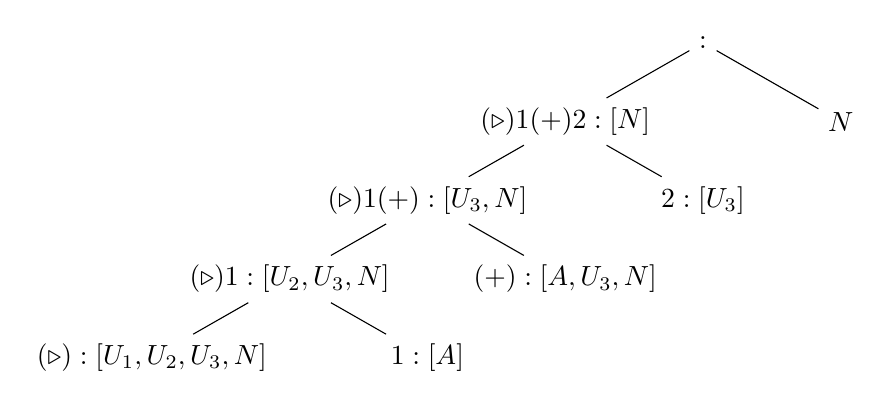
\begin{tikzpicture}
    \def\app{{\scriptsize app}}
    \def\f{{(\triangleright)}}
    \def\p{{(+)}}
    \node {:} [sibling distance = 3.5cm, level distance = 1cm]
        child {node {$\f 1 \p 2:[N]$}
            child {node {$\f 1 \p:[U_3, N]$}
                child {node {$\f 1:[U_2, U_3, N]$}
                    child {node {$\f: [U_1,U_2,U_3,N]$}}
                    child {node {$1: [A]$}}
                }
                child {node {$(+): [A,U_3,N]$}}
            }
            child {node {$2: [U_3]$}}
        }
        child {node {$N$}};
\end{tikzpicture}
}

We start with the elaboration of $(\triangleright) 1 (+) 2$ with the signature
requirement $[N]$ and the required type $N$.

\begin{itemize}
    \item The term is an application with the function term $(\triangleright) 1
        (+)$ and the argument $2$. We start the elaboration of the function term
        with the signature requirement $[U_3, N]$ and no required type.

    \item The term is again an application with the function term
        $(\triangleright) 1$ and the argument $(+)$. We start the elaboration
        of the function term with the signature requirement $[U_2, U_3, N]$ and
        no required type.

    \item The term is again an application with the function term
        $(\triangleright)$ and the argument $1$. We start the elaboration of the
        function term with the signature requirement $[U_1, U_2, U_3, N]$ and no
        required type.

    \item The term $(\triangleright)$ is a global name with the signature $[I,
        I, A, [A, P], P]$. Unification with the required signature $[U_1, U_2,
        U_3, N]$ results in
        $$
        \begin{array}{lll}
            U_1 &:=& A
            \\
            U_2 &:=& [A, U_3, N]
            \\
            P   &:=& [U_3, N]
        \end{array}
        $$
        Because of the two implicit arguments the term is elaborated as
        $(\triangleright)A P$ with the metavariables $A$ and $P$.

    \item Next the argument term $1$ has to be elaborated with the required
        signature $[A]$ and the required type $A$. This elaboration gets stuck
        on $A$, because the elaborator cannot decide the number type.

    \item Next the argument term $(+)$ is tried with the required signature $[A,
        U_3, N]$. The global name is ambiguous, but the ambiguity can be
        resolved by the result type. The signature is $[N, N, N]$. Unification
        with the required signature results in
        $$
        \begin{array}{lll}
            A &:=& N
            \\
            U_3 &:=& N
        \end{array}
        $$

    \item Now the complete term can be elaborated as
        $$
            (\triangleright) N (N \to N) \meta a (+) \meta b
        $$
        leaving the two holes $\meta a$ and $\meta b$ for the remaining
        arguments. However by unification the metavariables $\meta A$ and $\meta
        U_3$ are instantiated by $N$ and therefore the elaboration of the
        remaining arguments is unblocked and finally will succeed.
\end{itemize}


\section{Bound Variables}

The function type

$$
\Pi x^A. R
$$

has a bound variable $x$ of type $A$ and a result type $R$ which might depend on
$x$.

A bound variable has the following attributes.

\begin{enumerate}

    \item Implicit: Let $f: \Pi x^A. R$ be a function and $f a$ an application.
        If the bound variable is implicit, then the compiler is instructed to
        infer the argument $a$ from the context in case it is missing.

    \item Dependent: A variable is dependent if the result type depends on it.

        Open point: What happens in
        $$
            \Pi P^{A \to \Any} x^A. P x
        $$
        if $P = \lambda x^A . N$? Is $x$ dependent?

    \item Ghost: A ghost variable means that its value cannot be used in the
        runtime code. It can be

        \begin{itemize}
            \item used in types

            \item used as an argument to a function which expects a ghost argument

            \item pattern matched on to make decisions if the result type of the
                decision is a proposition

            \item used as an argument to any function whose return type is a
                propositon.

        \end{itemize}
\end{enumerate}

A term which is not a type (i.e. its type is not a sort) are propositional or
non-propositional. A term is propositional if its type is a proposition.
Otherwise it is non-propositional. Non-propositional terms represent potential
runtime objects.

If a constructor for a proposition uses non-propositional bound variables, then the
non-propositonal bound variable is a ghost variable. A pattern match uncovering
it can use its value only as a ghost value. A decision cannot be made on pattern
match unless the result type of the pattern match is a proposition.


\section{Universes}





\subsection{Universes and Sorts}
%%%%%%%%%%%%%%%%%%%%%%%%%%%%%%%%%%%%%%%%%%%%%%%%%%%%%%%%%%%%%%%%%%%%%%%%%%%%%%%%


We have the following sorts or universes (sorts and universes are synonymous):
\begin{enumerate}
\item $\Prop$: Impredicative universe of propositions

\item $\Any_i$: Predicative universes of types for $i \in \set{0, 1, 2, \ldots}$

\item $\Any_\infty$: Top universe
\end{enumerate}
and the builtin type $\Uni$ with the typing judgements which are treated as
axioms:
$$
\begin{array}{l}
    \Uni : \Any_\infty
    \\
    \Prop : \Any_0 : \Any_1 \ldots
\end{array}
$$


All sorts except the top sort $\Any_\infty$ have types. Therefore it is
possible to introduce type variables $X: s$ for all sorts except the top sort.

Furthermore since $\Uni$ has type $\Any_\infty$ it is possible to introduce
universe variables $u: \Uni$.

The type of a type is always a sort. The sort of a type defines the
universe of the type. I.e. all types live in a universe. The typing judgement
$T: s$ says that the type $T$ lives in the universe $s$.


There is a subtle difference between the universe of a type and the universe of
an object. An object has a type and its type lives in a universe. We say the an
\emph{object $o$ lives in a universe $s$ if its type $T$ lives in the universe
$s$}. I.e. the typing judgement $o : T : s$ must be valid. In other words $o$
has type $T$ and $T$ has type $s$.

A type $T$ can be regarded as a type. Then its type is a sort $s$ with $T : s$
and it therefore lives in the universe $s$ as a type.

However a type can be regarded as an object as well. Then there is the typing
judgement $T: s_1 : s_2$. We say the object $T$ lives in the universe $s_2$.

Some examples: The type $\Nat$ lives in the universe $\Any_0$. The object $1$
has type $\Nat$. Therefore the object $1$ lives in the universe $\Any_0$. The
object $\Nat$ has type $\Any_0$ which has the type $\Any_1$. Therefore the
object $\Nat$ lives in the universe $\Any_1$. By the same reasoning the object
$\Any_0$ lives in the universe $\Any_2$.

All types regarded as objects live in a universe higher than the types regarded
as types.




\subsection{Typing Rules}
%%%%%%%%%%%%%%%%%%%%%%%%%%%%%%%%%%%%%%%%%%%%%%%%%%%%%%%%%%%%%%%%%%%%%%%%%%%%%%%%


Typing rules for products:
\begin{enumerate}
    \item Propositional Products:
        $$
            \rulev{
                \Gamma \vdash A: s
                \\
                \Gamma, x^A \vdash B: \Prop
                \\
                A \ne \Uni
            }
            {
                \Gamma \vdash \Pi x^A. B : \Prop
            }
        $$
    \item Predicative Products:
        $$
            \rulev{
                \Gamma \vdash A: \Any_i
                \\
                \Gamma, x^A \vdash B: \Any_i
            }
            {
                \Gamma \vdash \Pi x^A. B : \Any_i
            }
        $$

    \item Universe Products:
        $$
            \rulev{
                \Gamma \vdash u: \Uni
                \\
                \Gamma, u^\Uni \vdash B: s
                \\
                A \ne \Uni
            }
            {
                \Gamma \vdash \Pi u^\Uni. B : \Any_\infty
            }
        $$
\end{enumerate}
These rules guarantee that the type $\Pi u^\Uni. B$ of a universe polymorphic
object cannot be used as an argument to a function.


Furthermore we have the cumulativity rule
$$
\rulev{
    \Gamma \vdash t : T
    \\
    \Gamma \vdash U : s
    \\
    T \le U
}
{
    \Gamma \vdash t : U
}
$$
The cumulativity rule for predicative universes says that whenever $T: \Any_i$
is valid, then $T: \Any_j$ is valid for all $i \le j$ since $\Any_i \le \Any_j$
is valid.  Together with the predicative product rule we get
$$
\rulev{
    \Gamma \vdash A: \Any_i
    \\
    \Gamma, x^A \vdash B: \Any_j
    \\
    i \le k
    \\
    j \le k
}
{
    \Gamma \vdash \Pi x^A.B : \Any_k
}
$$
or maybe more specific
$$
\rulev{
    \Gamma \vdash A: \Any_i
    \\
    \Gamma, x^A \vdash B: \Any_j
}
{
    \Gamma \vdash \Pi x^A.B : \Any_{\text{max}(i,j)}
}
$$






\subsection{Constraints}
%%%%%%%%%%%%%%%%%%%%%%%%%%%%%%%%%%%%%%%%%%%%%%%%%%%%%%%%%%%%%%%%%%%%%%%%%%%%%%%%


Universe variables are always implicit. The programmer usually ommits universe
variables in the source code i.e. instead of $\Any_u$ the source code contains
only $\Any$. The compiler generates for each sort $\Any$ in the source code a
metavariable $\meta u : \Uni$ and interprets the sort $\Any$ as $\Any_{\meta
u}$.

There are the following two sources of constraints between universes.

\begin{enumerate}
    \item Predicative type argument $T: \Any_{u}$: If $T$ is used as an actual
        argument e.g. in the expression $f T$, then the function $f$ must have
        the type $\Pi X^{\Any_v}. R$.  This creates the constraint $u \le v$.

    \item Predicative inductive type $\Pi \vec x^{\vec A}. \Any_{v}$: Any
        instance of such an inductive type lives in the universe $\Any_{v}$.

        This requires that all arguments of all contructors must not live in a
        higher universe. Reason: Pattern matches of an indutive type living in
        the universe $\Any_{v}$ must not uncover any object living in a
        higher universe. In other words: \emph{Only smaller (or equal) things
        can be used to create greater things}.

        I.e. any constructor argument living as an object in the universe
        $\Any_u$ creates the constraint $u \le v$.
\end{enumerate}






\subsection{Predicative Inductive Types}
%%%%%%%%%%%%%%%%%%%%%%%%%%%%%%%%%%%%%%%%%%%%%%%%%%%%%%%%%%%%%%%%%%%%%%%%%%%%%%%%

In Alba new types can be created as inductive types. The simplest inductive
types have neither parameter nor index arguments.
$$
\begin{array}{lll}
    B &:=& [T^{\Any_0} \mid T, T]
    \\
    N &:=& [T^{\Any_0} \mid N, N \to N]
\end{array}
$$

The types of booleans and natural numbers live in the universe $\Any_0$ because
of the typing judgements $B: \Any_0$ and $N: \Any_0$. Objects of type boolean do
not contain anything. Objects of type $N$ might contain other natural numbers
(second constructor). There is no possibility for such simple types to contain
objects living in a higher universe than $\Any_0$.

Polymorphic types like lists and pairs have type parameters. The type parameters
can live in any universe. Therefore they need an universe level parameter and a
type parameter whhich depents on the uinverse level.

$$
\begin{array}{lllll}
    L &:=& [i^\Uni, A^{\Any_i} &\mid T^{\Any_i} &\mid T, A \to T \to T]
    \\
    P &:=& [i^\Uni, A^{\Any_i}, B^{\Any_i} &\mid T^{\Any_i} &\mid A \to B \to T]
\end{array}
$$

Having that we can construct a list of natural numbers $L\,0\,N: \Any_0$ living
in the universe level $0$. However it is possible to construct list of types
$L\,(i+1)\,\Any_i$ which might live in the universe level $i$. The types as
types live in the universe level $i$, but the types as objects live in the
universe level $i+1$. Therefore the whole list which contains objects from the
universe level $i + 1$ lives in the universe level $i+1$ as well.


A more complex type is the dependent list.
$$
\begin{array}{lllll}
    \text{DL} &:=&
    [
        i^\Uni, A^{\Any_i}, P^{A \to \Any_i}
        &\mid
        T^{LiA \to \Any_i}
        &\mid
        T[],
        \Pi a^A \text{as}^{LiA}.
            Pa \to T\text{as} \to T(a :: \text{as})
    ]
\end{array}
$$

A dependent list might contain objects of type $A$, $LiA$, $Pa$ and
$T\text{as}$. All these object live in the universe level $i$. Therefore the
whole dependent list can live in the universe level $i$.

Furthermore we can construct hetergeneous lists.
$$
\begin{array}{lllll}
    \text{HL} &:=&
    [
        i^\Uni
        &\mid
        T^{L(i+1)\Any_i \to \Any_{i+1}}
        &\mid
        T[],
        \Pi A^{\Any_i} \text{As}^{L(i+1)\Any_i}.
            A \to T\text{As} \to T(A :: \text{As})
    ]
\end{array}
$$
A heterogeneous list contains objects $A$ and $\text{As}$ with the typing
judgements $A : \Any_i : \Any_{i+1}$, $\text{As}: L(i+1)\Any_i : \Any_{i+1}$.
These objects live in the universe level $i+1$. Therefore the whole
heterogeneous list object must live in the universe level $i+1$ as well.


Here is a rather strange type
$$
\begin{array}{lllll}
    \text{Ex}
    &:=&
    [
        i^\Uni,
        P^{\Any_i \to \Prop}
        &\mid
        T^{\Any_{i+1}}
        &\mid
        \Pi X^{\Any_i}. P X \to T
    ]
\end{array}
$$




\subsection{No Universe Polymorphism}
%%%%%%%%%%%%%%%%%%%%%%%%%%%%%%%%%%%%%%%%%%%%%%%%%%%%%%%%%%%%%%%%%%%%%%%%%%%%%%%%

No universe polymorphis means that all user entered $\Any$ are interpreted as
$\Any_0$. Therefore all types live as types at the universe level $0$ and all
objects which are not types live as well at the universe level $0$. Types as
objects live at the universe level $1$.

This has an important consequence: \emph{Type objects cannot be contained within
other objects}. There is no list of types, no pair of types etc.

Of the above examples nearly all types are possible without universe
polymorphism. Only heterogeneous lists $\text{HL}$ and the strange type
$\text{Ex}$ are not possible without universe polymorphism.

Without universe polymorphism we are basically in the calculus of constructions
with inductive types. All construction which require an infinite set of
stratified universes with cumulativity are not possible.


\end{document}
